\documentclass[prb,preprint]{revtex4-1} 
\raggedbottom
\usepackage{amsmath}
\usepackage{amsfonts}
\usepackage{graphicx}

\begin{document}

\section{Optical Pumping Results and Analysis}

After canceling out the the earth's magnetic field we begin pumping Rb atoms into a transparent state. At this point we take voltage versus time data which represents Rb population oscillations following that pumping. Using a least squares optimization of the function
\begin{equation}\label{per}
A\text{cos}(\omega t+\delta)e^{t/\tau}+B
\end{equation}
where $A$, $\delta$, $\tau$, and $B$ are arbitrary constants and $2\pi/\omega$ represents the frequency of the oscillations. For $^{85}$Rb and $^{87}$Rb respectively, Tables \ref{tab1} and \ref{tab2} show voltages which correspond to RF field strengths, or amplitudes, at a frequency $f_0$ of 151.400$\pm$0.001 kHz. They also show the correlated frequency $f$ of the dampened oscillations for each isotope which is determined by fitting the aforementioned voltage vs time data to Eq \eqref{per} as shown in Fig \ref{LC}, where $2\pi/\omega=f$. We then make a simple linear fits of the two sets of data as shown in Fig \ref{ratio} to take a ratio of their slopes; the value of which should represent the ratio of the g-factors for $^{87}$Rb and $^{85}$Rb. It would also be appropriate to plot these data points with respect to the field strength, however since the voltage is proportional to it, such a calculation is not relevant when determining ratios.

\begin{table}[h!]

\begin{minipage}[b]{70mm}
\caption{Amplitude and $f$ for $^{85}$Rb}
\begin{ruledtabular}
\begin{tabular}{c c}
Amplitude (V) & $f$ (1/s)\\
\hline
0.66$\pm$0.02 & 473.5$\pm$0.3\\
1.06$\pm0.02$ & 783.1$\pm$0.5\\
1.34$\pm0.02$ & 996.0$\pm$0.7\\
0.94$\pm$0.02   & 682.6$\pm$0.5\\
0.58$\pm0.02 $  & 462.3$\pm$0.3\\
0.46$\pm0.02 $  & 333.7$\pm$0.2\\

\end{tabular}
\label{tab1}
\end{ruledtabular}

\end{minipage}
\begin{minipage}[b]{70mm}
\caption{Amplitude and $f$ for $^{87}$Rb}
\begin{ruledtabular}
\begin{tabular}{c c}
Amplitude (V) & $f$ (1/s)\\
\hline
0.512$\pm$0.02 & 570$\pm$5\\
0.713$\pm0.02$ & 778$\pm$1\\
0.941$\pm0.02$ & 1021$\pm$4\\
1.15$\pm$0.02   & 1279$\pm$70\\
1.36$\pm0.02 $  & 1481$\pm$4\\
--------  & --------\\
\end{tabular}
\end{ruledtabular}
\label{tab2}
\end{minipage}

{Tables \ref{tab1} and \ref{tab2} show RF field strengths in terms of voltage, at $f_0$ as they compare to $f=1/T$.}
\end{table}

\begin{figure}[h!]
\centering
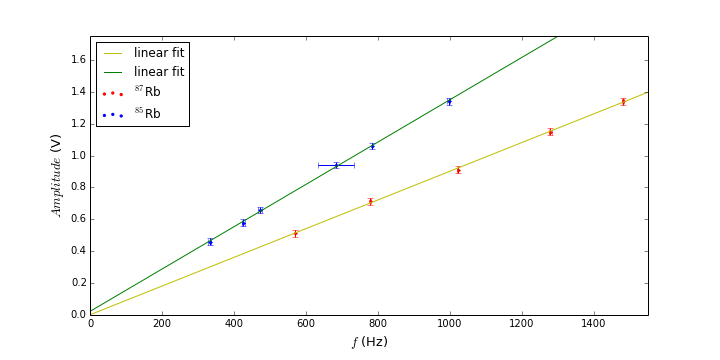
\includegraphics[width=0.9\textwidth]{ratios.png}
\caption{A plot of $f$ vs $V$ for $^{87}$Rb and $^{85}$Rb with trend lines.}
\label{ratio}
\end{figure}

\begin{figure}[h!]
\centering
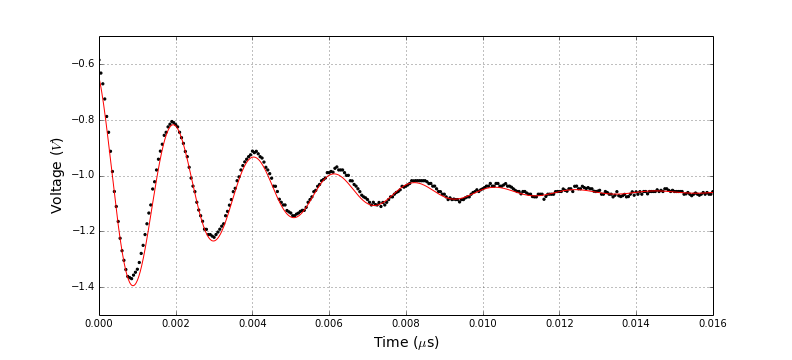
\includegraphics[width=0.9\textwidth]{per_fit.png}
\caption{Fit of voltage versus time data using a damped oscillation function of the form of Eq \ref{per}}
\label{LC}
\end{figure}

\newpage
The ratio of $^{87}$Rb's trend line to $^{85}$Rb's in Fig \ref{ratio} was found to be $0.67\pm0.01$ which corresponds well to the known value of 2/3. It should be noted though that in Table \ref{tab2} one measurement of $f$ has a significantly higher degree of uncertainty than the others; this is because it was not possible to fit Eq \eqref{per} to the data. Instead the frequency for this data point was simply estimated.

Following this, we then fit another set of voltage versus time data using a least squares optimization of a simple exponential decay function. With this function we were able to determine the time constant, or the optical pumping time which was used during the experiment. This time was determined to be 0.9009$\pm0.001\times10^{-2}$ seconds. Fig \ref{LC1} shows a graph of the raw data along with the best fit line from which this values is derived. Note that the data in this figure has been rotated by 180 so that it will fit a typical exponential function.

\begin{figure}[h!]
\centering
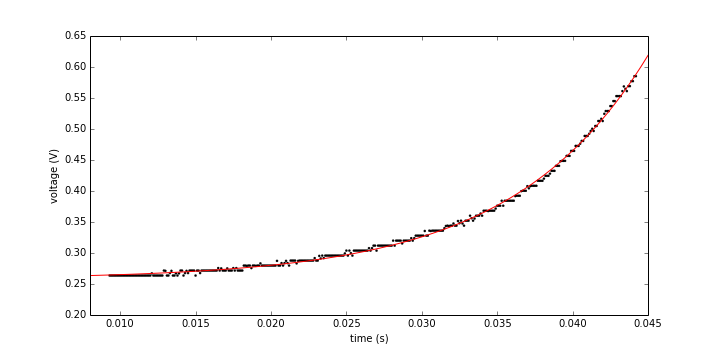
\includegraphics[width=0.9\textwidth]{exp_fit.png}
\caption{Fit of voltage versus time data which is used to determine the time constant using a simple exponential fit function.}
\label{LC1}
\end{figure}

Finally we collected data on the strength of the magnetic field acting on the $^{85}$Rb and  $^{87}$Rb isotopes along with the frequency at which resonance is achieved. This is all done in order to determine their respective $g$-factors. Fig \ref{LC2} demonstrates how these resonant frequencies were measured. In the end using the relationship $E=g_fm_f\mu_BB$ we found that the value for the two $g$-factors were $0.33\pm$0.02 and 0.42$\pm$0.02 respectively. The measured value for $^{85}$Rb compliments the accepted value of 1/3 while the value for $^{87}$Rb contrasts with the accepted values of 1/2. 

\newpage
\begin{figure}[h!]
\centering
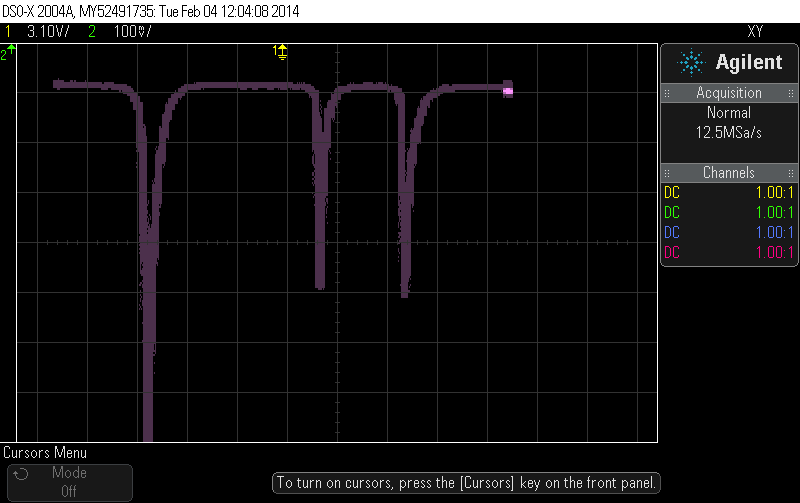
\includegraphics[width=0.9\textwidth]{scope_0.png}
\caption{A sample oscilloscope trace illustrating the zero-field resonance and RF resonances due to $^{87}$Rb and $^{85}$Rb}
\label{LC2}
\end{figure}
\newpage

\section{conclusion}
Though our values of $0.16361\pm$0.01 and 0.2105$\pm$0.01 for the $g$-factors for $^{85}$Rb and  $^{87}$Rb were far from expected, they were not entirely unreasonable if we consider the possible sources of error; Based on comments from other groups, and our own late observation, it appeared that the floor had a slight tilt to it which may have influenced our result. Give the sensitivity which optical pumping allows this seem like a likely culprit since the values are not obsene.

\end{document}